
\documentclass[a4paper]{article}

%%%%%%%% CREATE DOCUMENT STRUCTURE %%%%%%%%
%% Language and font encodings
\usepackage[english]{babel}
\usepackage[utf8x]{inputenc}
\usepackage[T1]{fontenc}
%\usepackage{subfig}

%% Sets page size and margins
\usepackage[a4paper,top=3cm,bottom=2cm,left=2cm,right=2cm,marginparwidth=1.75cm]{geometry}

%% Useful packages
\usepackage{svg}
\svgsetup{
    inkscape=pdf
}
\usepackage{amsmath}
\usepackage{amssymb}
\usepackage{graphicx}
% \usepackage[colorinlistoftodos]{todonotes}
\usepackage[colorlinks=true, allcolors=blue]{hyperref}
\usepackage{caption}
\usepackage{subcaption}
\usepackage{sectsty}
\usepackage{float}
\usepackage{titling} 
\usepackage{blindtext}
\setlength{\marginparwidth}{2cm}
\usepackage{todonotes}
\usepackage{csquotes}
\usepackage[
backend=biber,
style=numeric,
sorting=none
]{biblatex}
%\addbibresource{references.bib}
%\addbibresource{ref.bib}

\usepackage{xcolor}
\definecolor{darkgreen}{rgb}{0.0, 0.4, 0.0}
\setlength{\parindent}{0pt}

%%%%%%%% DOCUMENT %%%%%%%%
\begin{document}

%%%% Title Page
\begin{titlepage}

\newcommand{\HRule}{\rule{\linewidth}{0.5mm}} 							% horizontal line and its thickness
\center 
 
% University
\textsc{\LARGE Delft University of Technology}\\[1cm]

% Document info
									% Course Code
\HRule \\[0.8cm]
{ \huge \bfseries Bi-threshold Gates for Mechanical Logic in Intelligent Metamaterials }\\[0.7cm]								% Assignment
\HRule \\[2cm]
\large
\emph{Authors:}\\
Eoinlee Bley (5216737)\\[1.5cm]	
\emph{Supervisors:}\\
Dr. Davood Farhadi Machekposhti\\
Malte ten Wolde\\[0.5cm]
% Author info
in partial fulfillment of the requirements for the degree of \\[0.5cm]
\textbf{Master of Science}\\
in Mechanical Engineering\\[0.5cm]
{\large \today}\\[5cm]
\includegraphics[width=0.6\textwidth]{images/TU_delft_logo.jpg}\\[1cm] 	% University logo
\vfill 
\end{titlepage}

\begin{abstract}

\end{abstract}

\tableofcontents
\include{Preface}
\section{Introduction}
\label{sec:introduction}
\section{Results \& Discussion}

\subsection*{Elementary Cellular Automata Formalism}
Cellular automata (CA) are grid-based computational models where each cell evolves over time according to a rule set \( R \). In Elementary Cellular Automata (ECA), the domain is one-dimensional and the state space is binary, \( S = \{0, 1\} \). Each cell's future state is determined by its current state and those of its immediate neighbours.

Mathematically, for cell \( i \) at time \( t \), the next state \( u_i^{t+1} \) is governed by a rule function \( f: S^3 \to S \):

\[
u_i^{t+1} = f(u_{i-1}^t, u_i^t, u_{i+1}^t)
\]

With a binary state and 3-cell neighbourhood, there are \( 2^8 = 256 \) unique ECA rules. These are indexed from 0 to 255, following Wolfram's convention, detailed in \autoref*{sec:Wolfram Numbering Scheme for ECA}.

For example, Rule 110 is defined explicitly as:
\[
\begin{array}{ll}
f_{\text{110}}: & (0,0,0) \to 0, \; (0,0,1) \to 1, \; (0,1,0) \to 1, \; (0,1,1) \to 1, \\
& (1,0,0) \to 0, \; (1,0,1) \to 1, \; (1,1,0) \to 1, \; (1,1,1) \to 0
\end{array}
\]

Consult \autoref{fig:cube}A for a graphical depiction of Rule 110's eight possible neighbourhoods and their respective output states. Also shown is the time evolution of the rule, starting from a single 'on' cell at the left edge of the domain.

\subsection*{Hypercube Representation of Cellular Automata Rules}
Consider a cube in \( \mathbb{R}^3 \) as the domain \( D \), with each vertex representing a unique neighbourhood configuration \( N = (N_{-1}, N_0, N_1) \), where \( N_{-1}, N_0, N_1 \in \{0, 1\} \). The cube's vertices are colored based on a rule function \( f: \{0, 1\}^3 \to \{0, 1\} \), thereby geometrically realizing the Boolean truth table of an Elementary Cellular Automaton (ECA).

To introduce the concept of linear separability, consider separating parallel hyperplanes \( P \) defined by a normal vector \( \mathbf{n} \) and offsets \( \{d_1, d_2, \ldots, d_n\} \). These hyperplanes partition \( D \) into regions where the vertices share the same output state as determined by \( f \).

We define a domain classification function \( \Delta: D \to \{0, 1, \ldots, n\} \) as \( \Delta(x) = \sum_{i=1}^{n} H(\mathbf{n} \cdot \mathbf{x} - d_i) \), where \( H(z) \) is the Heaviside step function. Each value of \( \Delta(x) \) corresponds to one of the \( n+1 \) regions formed by \( P \).

Finally, a mapping function \( M: \{0, 1, \ldots, n\} \to \{0, 1\} \) translates the region identifier \( \Delta(x) \) into the 'on' or 'off' state for each neighbourhood configuration.
Refer to \autoref*{fig:cube}B for a graphical representation of the cube and separating planes for Rule 110.

As shown in Appendix \ref*{sec:Bi-planar separability of ECA rules}, most ECA rules are bi-planarly separable, i.e. they can be represented by two parallel planes. 


\begin{figure}[ht]
    
    \centering
    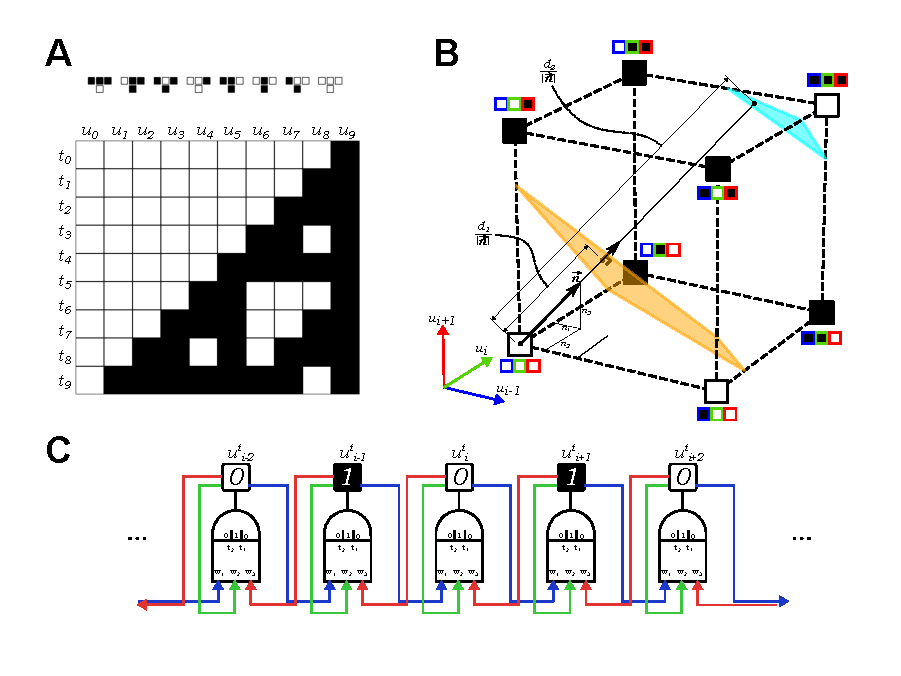
\includegraphics[width=\textwidth]{images/SVGs/Cube.pdf}
    \caption{A. The transition rule and time evolution of the Rule 110 cellular automata. B. Cube representation Rule 110 with separating planes defined by normal vector $\overrightarrow{n}$ and offset constants $d_1$ and $d_2$. The red, green and blue colouring corresponds to left neighbour, middle, and right neighbour cells of the neighbourhood respectively. C. Bi-threshold gate representation of an ECA architechture.}
    \label{fig:cube}
\end{figure}
\subsection*{Bi-threshold Gates}

The result of this formulation of 3-input Boolean functions as linearly separable regions in a cube is the observation that most 3-input Boolean functions can be represented by a pair of parallel planes. This means we can translate a complicated Boolean algebraic expression composed of several AND, OR, XNOR, etc., gates into a single bi-threshold perceptron gate.

The bi-threshold perceptron for this ECA context can be formally represented as:

\[
f(N) = \begin{cases} 
0 & \text{if } \sum_{i=-1}^{1} w_i \cdot N_i > T_1 \\
1 & \text{if } T_2 \leq \sum_{i=-1}^{1} w_i \cdot N_i \leq T_1 \\
0 & \text{if } \sum_{i=-1}^{1} w_i \cdot N_i < T_2
\end{cases}
\]


\subsection*{Concept Mechanism}

In light of the mathematical formalism presented, we introduce a conceptual mechanical metamaterial designed to embody the logic and behavior of Elementary Cellular Automata (ECAs). This metamaterial is constructed from an array of interconnected unit cells, each serving as a mechanical analog to the bi-threshold perceptron.

The core of each unit cell is a tristable element, functioning as the decision-making component. The tristable element has three stable states, akin to the three regions separated by the two parallel planes in the cube of our geometric representation. This element is responsible for holding the output state of the cell, dictated by the weighted sum of its inputs.

Each unit cell is interconnected via coupling springs, which transmit mechanical signals between adjacent cells. The stiffness values of the coupling springs \(k_i\) act as the weights \( w_i \) in the bi-threshold perceptron equation. These values determine the force interactions and state transitions between adjacent unit cells. The tristable elements have multiple stable states, analogous to the regions separated by planes in the cube of our geometric ECA representation.

An input clock signal introduces a temporal dimension to the mechanical system, enabling dynamic state evolution similar to time-stepping in ECAs. This clock signal sets the computational cycle and synchronizes the unit cells.

Thus, the mechanical properties of the springs and tristable elements correspond directly to the mathematical constructs of the bi-threshold perceptron, providing a means to implement ECA rules in a mechanical system. The specific embodiment of this concept is detailed in the following section.

\subsection*{Unit cell design}
The unit cell is designed to be planar and monolithic for scalability, operate under a single shared clock signal for synchronization, transmit forces between adjacent cells, hold state in the absence of input, and transition states according to neighboring conditions. \autoref*{fig:Mechanism} depicts the unit cell and its key components: the tristable element in teal, the bistable element in purple, the signal transmission element in orange, and the input bifurcation element in dark blue. Coupling springs, coloured in red, green, and blue, link the tristable element out-of-plane to the bifurcation elements of adjacent unit cells. The configuration of each unit cell is fully defined by two displacements: \(d^t\) in the \(\hat{e}_1\) direction for the tristable element and \(d^b\) in the \(\hat{e}_1\) direction for the bifurcation element. The input bifurcation element is so named because 

The bistable element acts as a mechanical binary memory element for the unit cell, while the tristable element's two snapthrough force thresholds act as decision boundaries corresponding to the thresholds of the threshold gate, or the separating planes of the boolean function. The signal transmision and bifurcation elements facilitate the temporal clocking and informational interconnection of the unit cells. 



\begin{figure}[h]
    \centering
    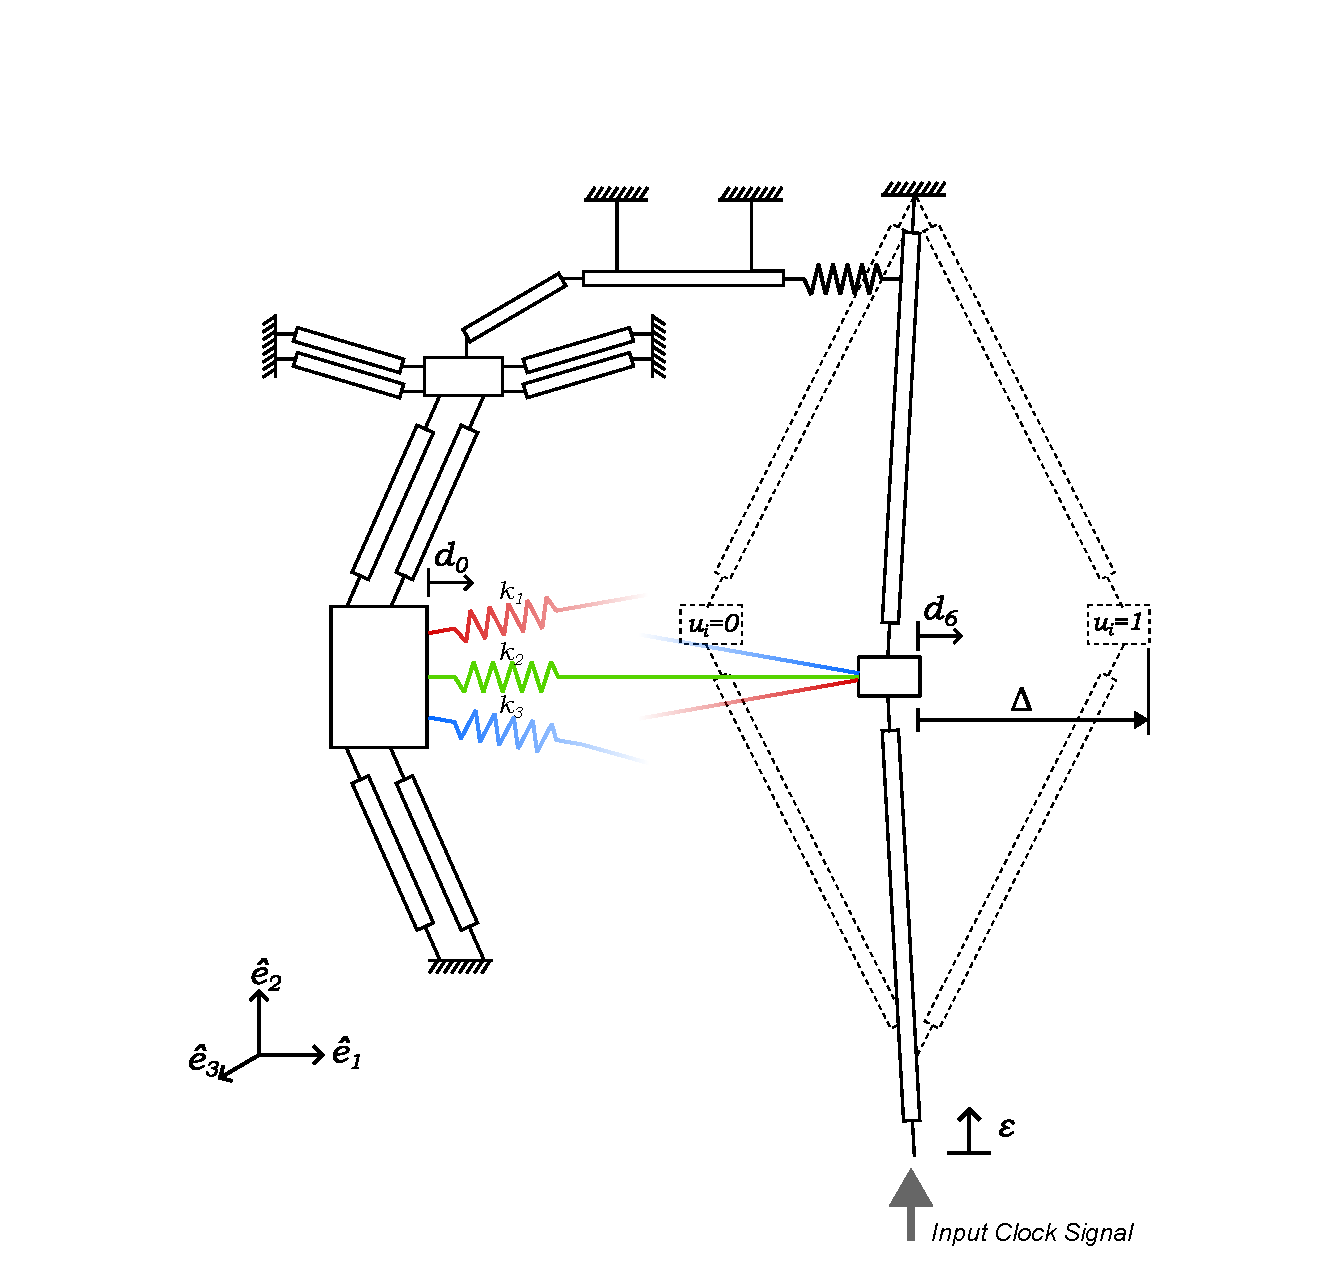
\includegraphics[width=\textwidth]{images/SVGs/PRBM.pdf}
    \caption{This is a figure.}
    \label{fig:Mechanism}
\end{figure}

\begin{figure}[h]
    \centering
    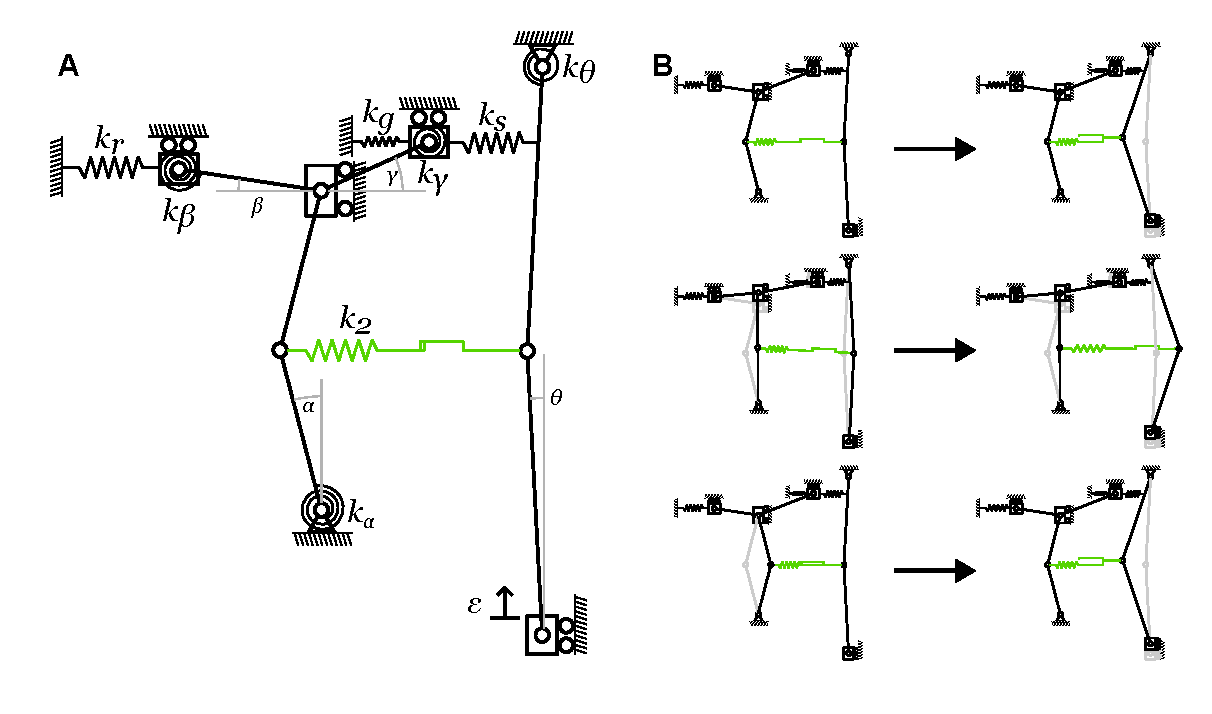
\includegraphics[width=\textwidth]{images/SVGs/Bifurcation_and_PRBM.pdf}
    \caption{This is a figure.}
    \label{fig:Bifurcation}
\end{figure}

\subsection*{Working Principle}
\begin{figure}[h]
    \centering
    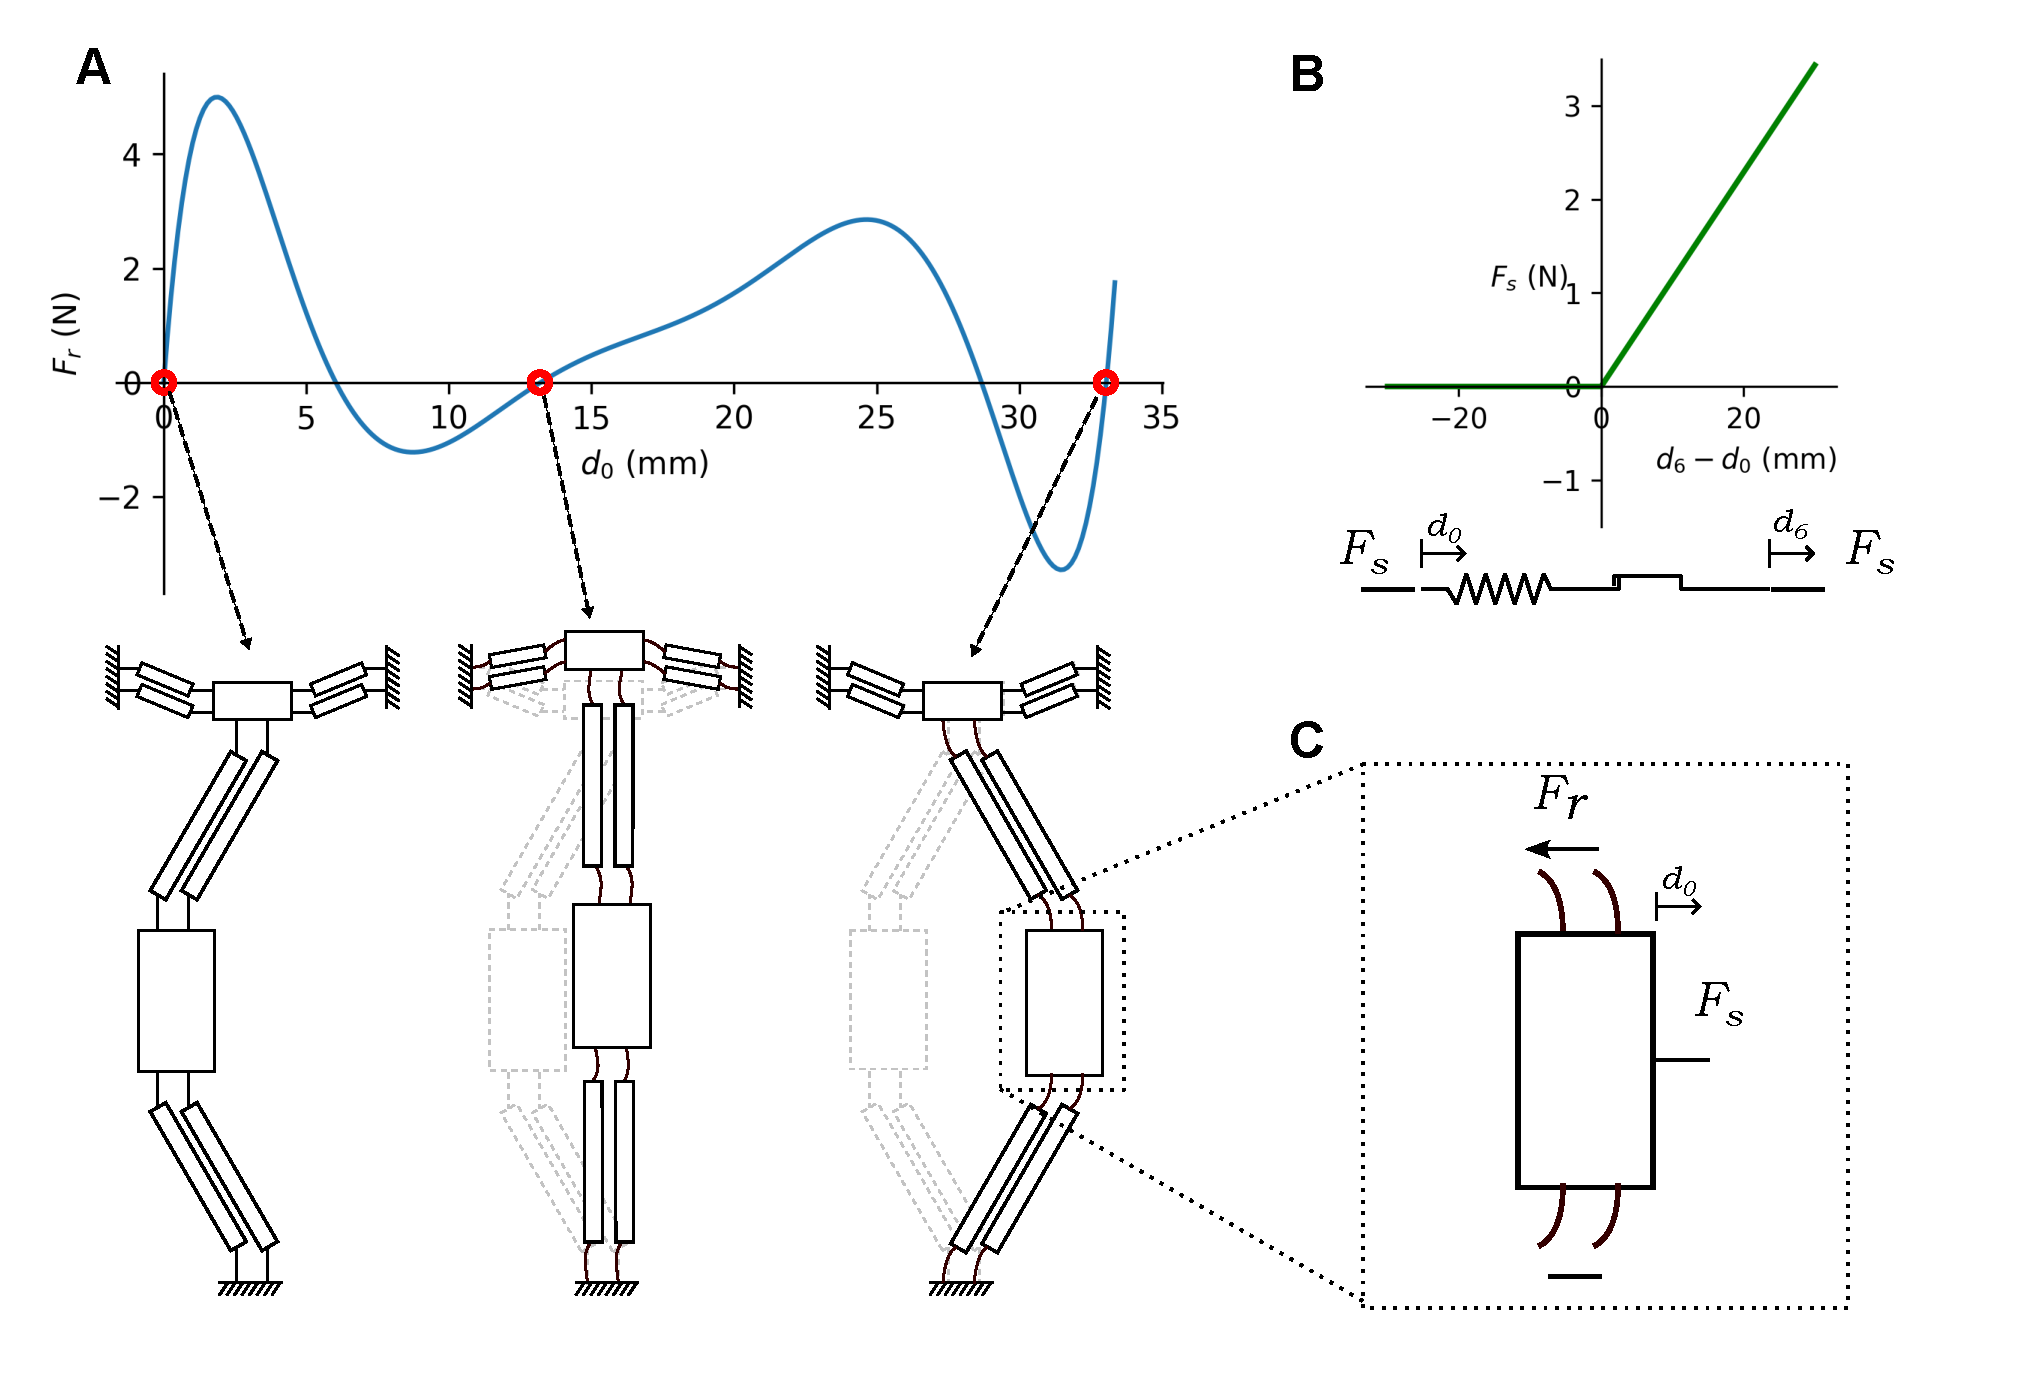
\includegraphics[width=\textwidth]{images/SVGs/Equilibria1.pdf}
    \caption{A. Force-displacement response of thethree stable equilibria and corresponding configurations of the state element. B. Force-displacement response of the tension only spring }
    \label{fig:Equilibria and Tension-only spring}

\end{figure}
    \todo{generate pdf of this figure and edit axis labels}
% \begin{figure}
%     \centering
%     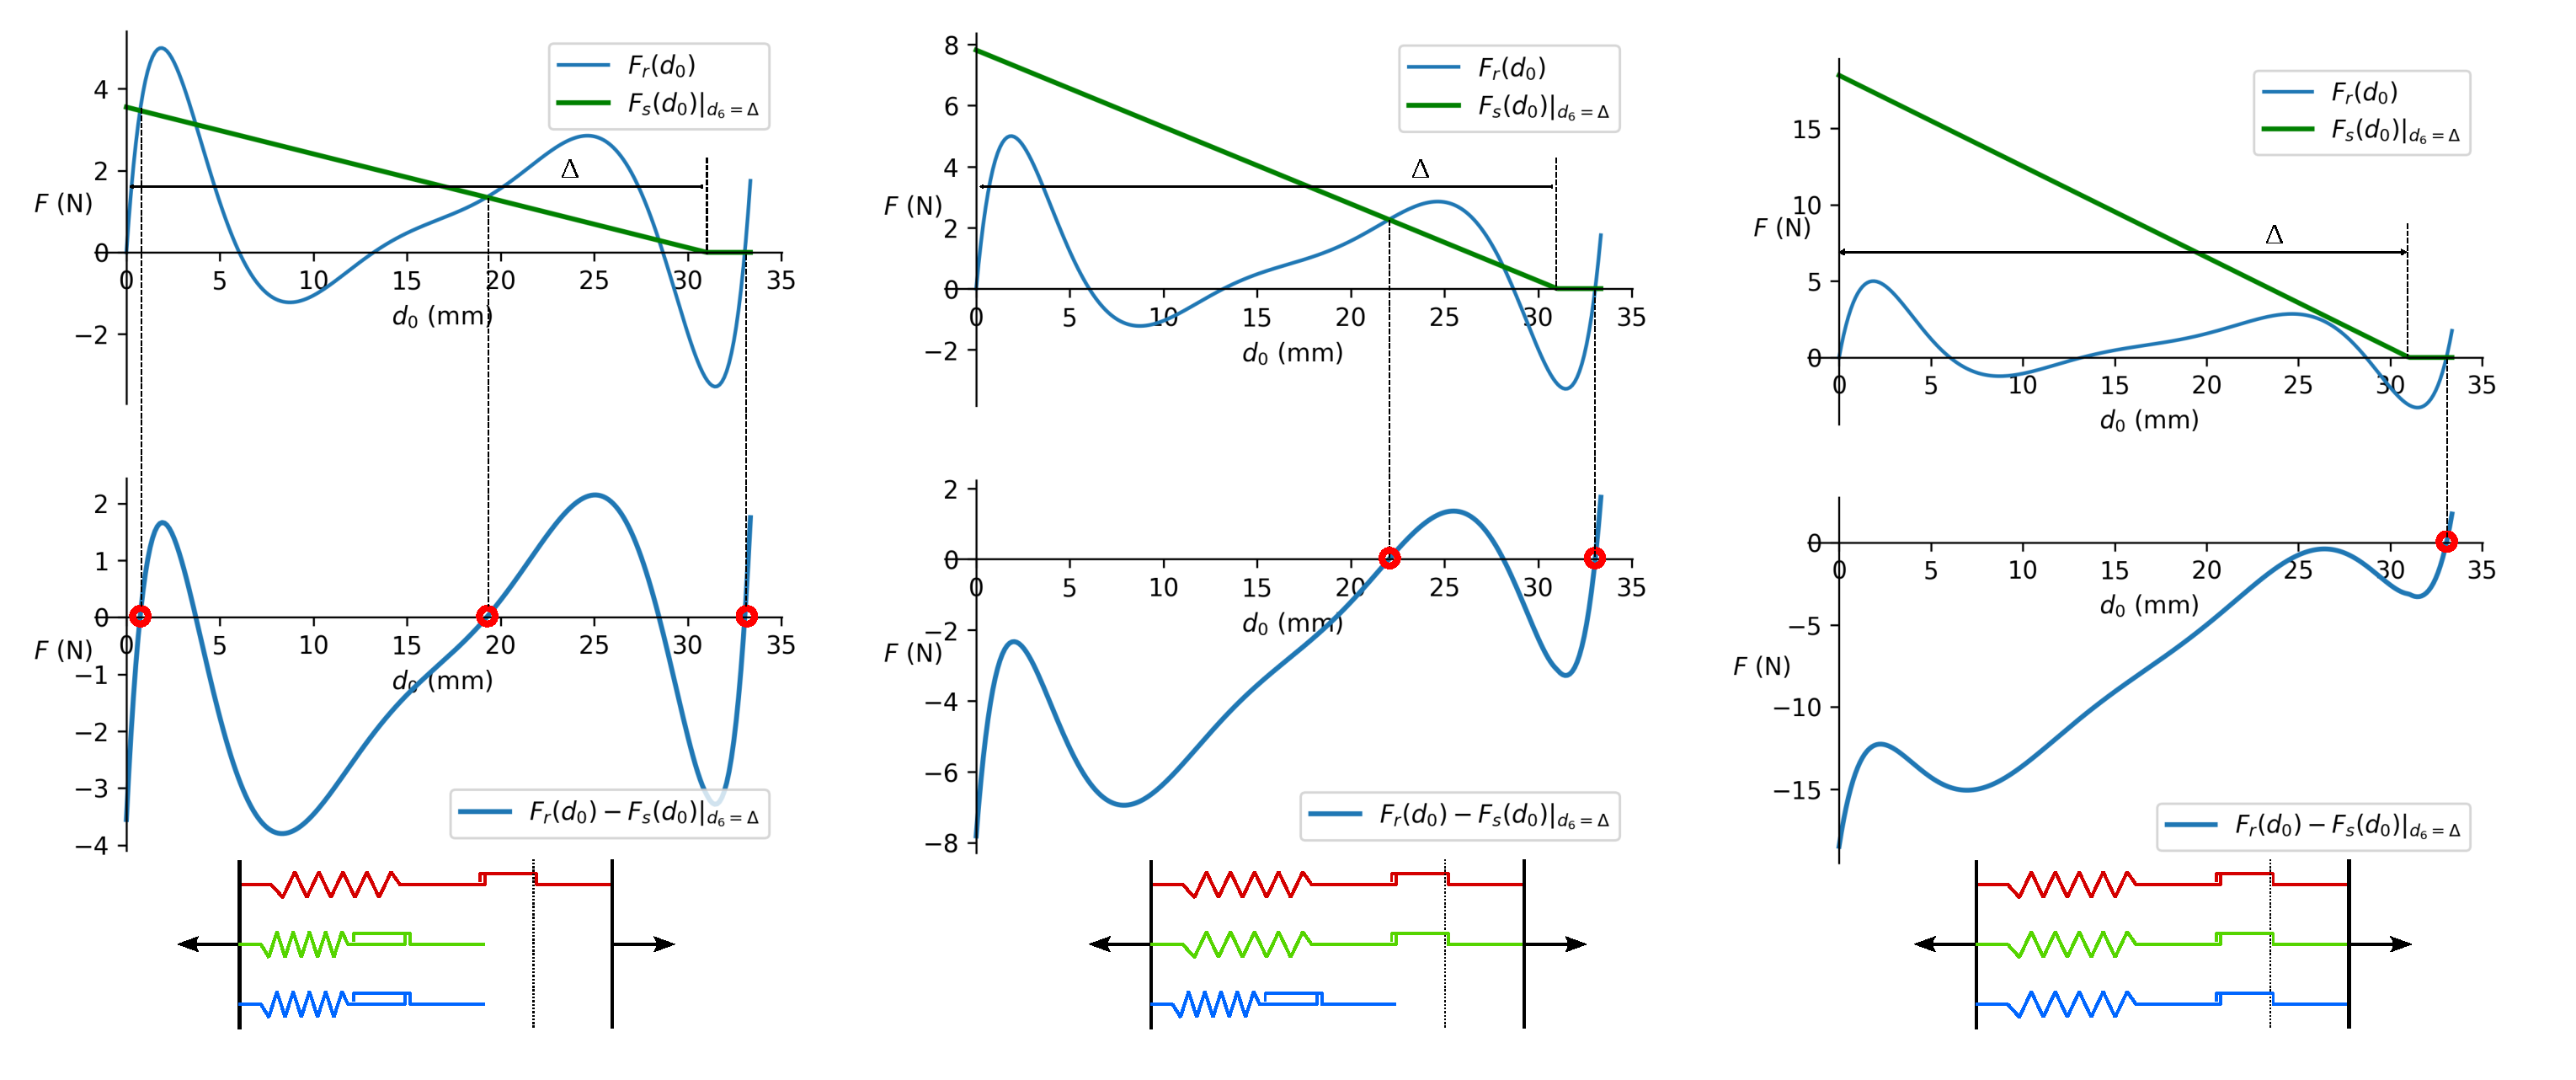
\includegraphics[width=\textwidth]{images/SVGs/Equilibria2.pdf}
%     \caption{This is a figure.}
%     \label{fig:Equilibria under actuation}
% \end{figure}

% \begin{figure}
%     \centering
%     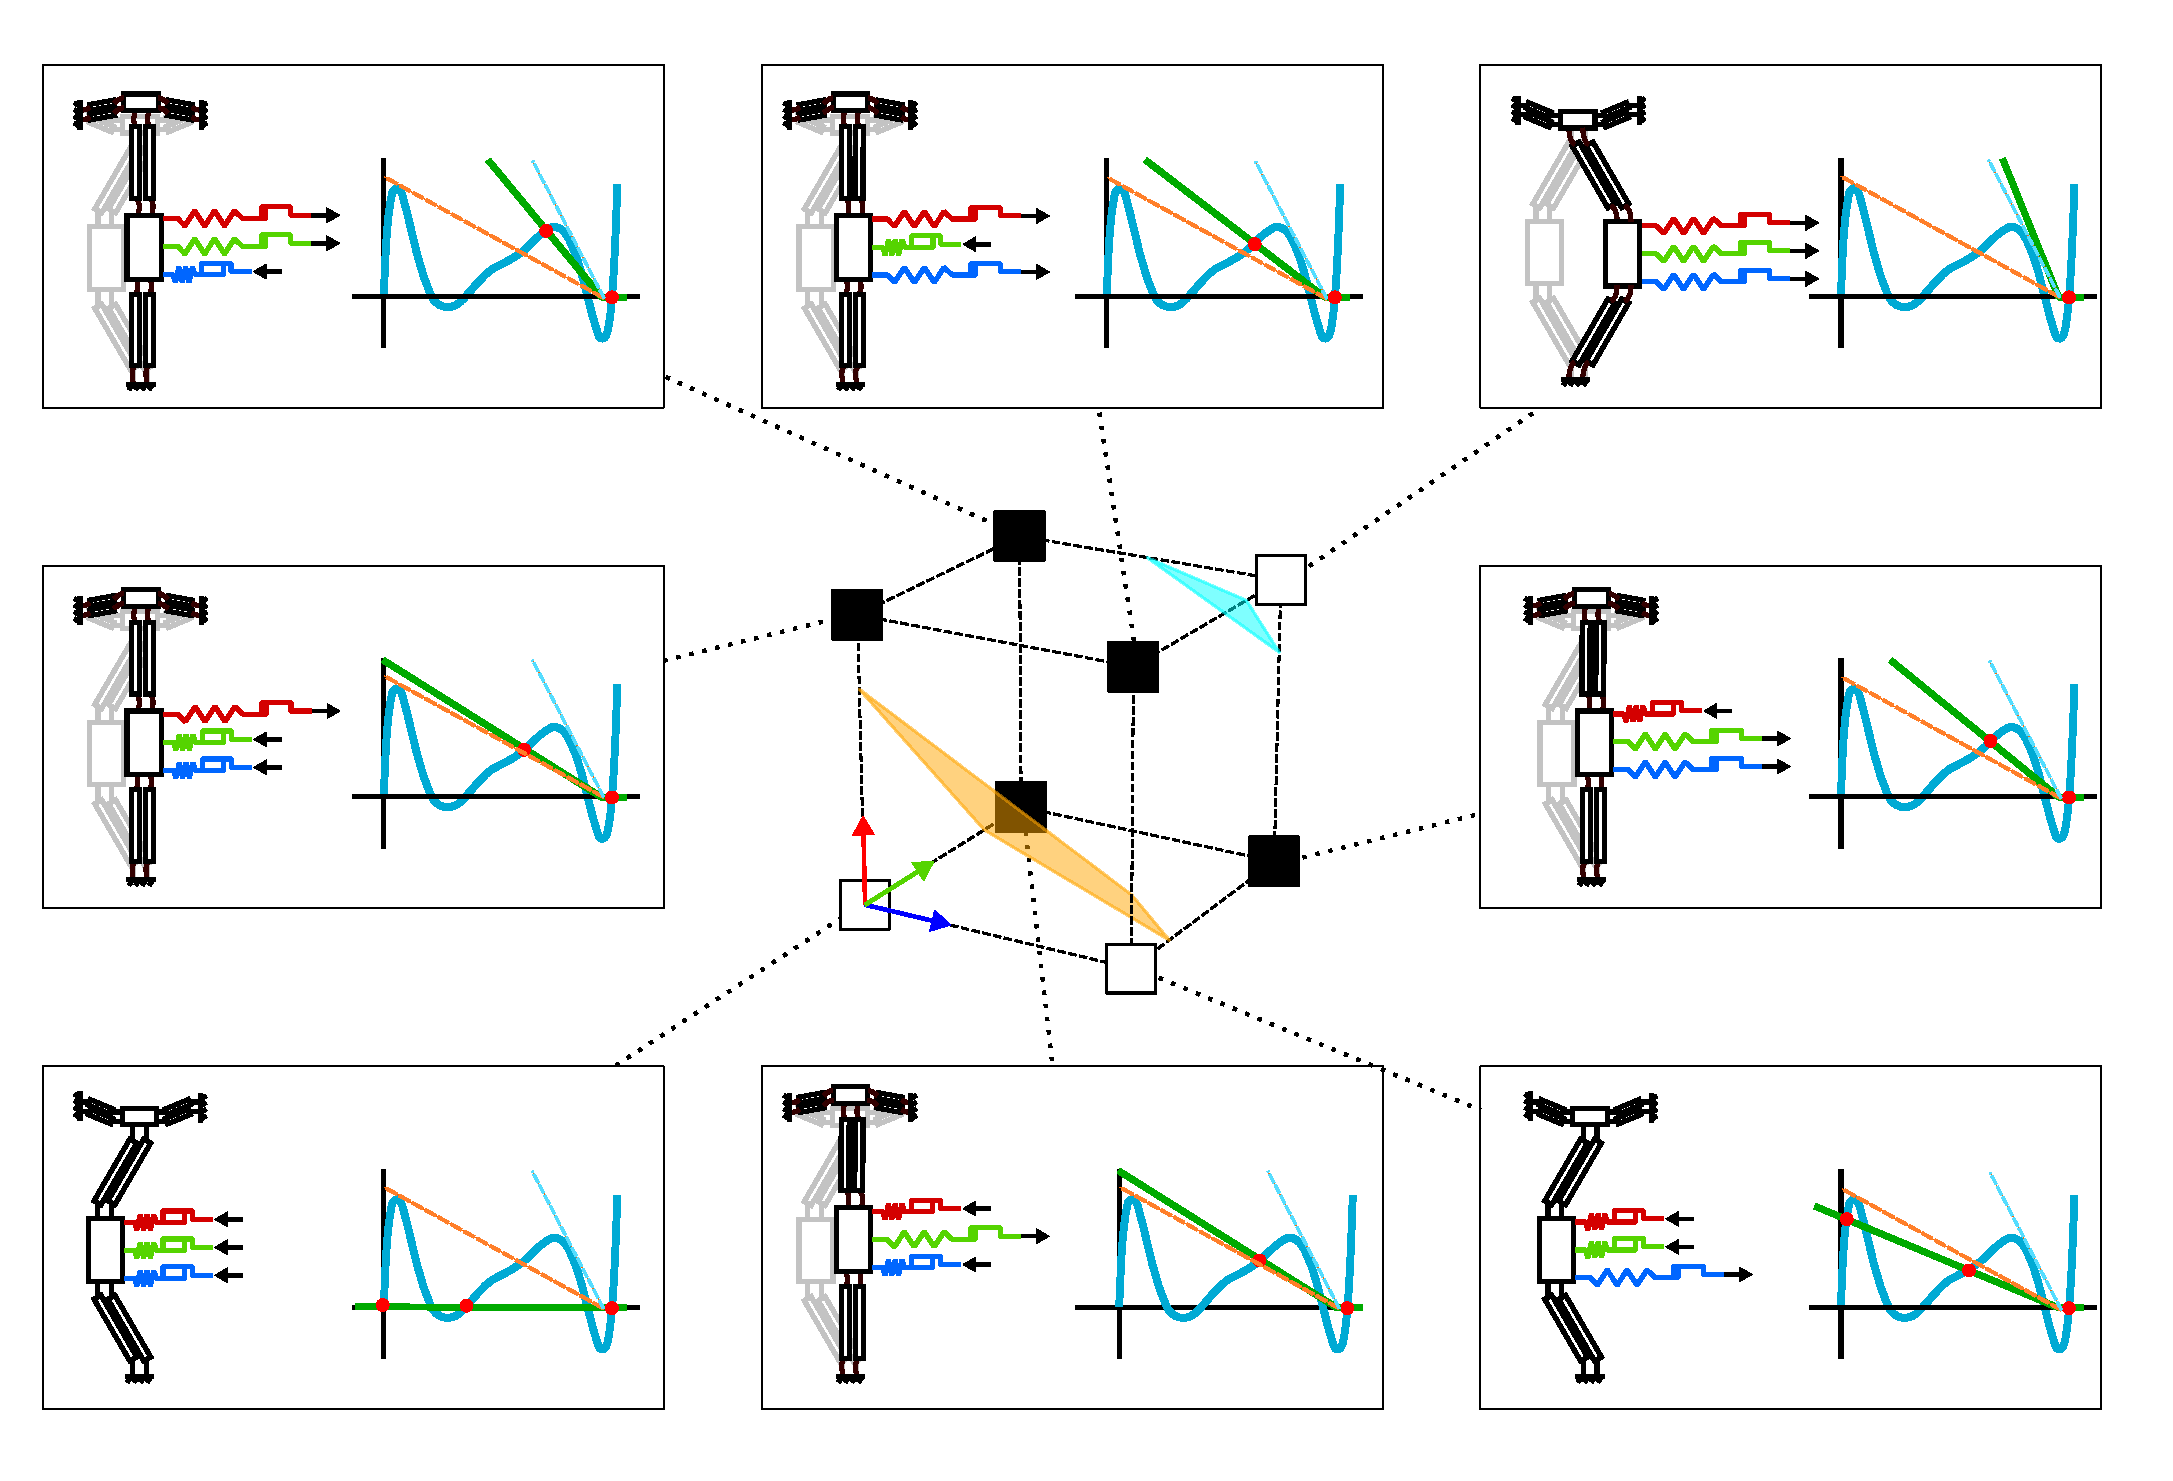
\includegraphics[width=\textwidth]{images/SVGs/Equilibria3.pdf}
%     \caption{This is a figure.}
%     \label{fig:Equilibria corresponding to Rule 110}
% \end{figure}

% \subsection*{Simulation}
% \section{Conclusion}
% \section{References}
\appendix
\section{Supplementary Material}
%%%% SECTIONS
%% Section 1

\newpage

\begin{figure}
    \centering
    \includesvg[width=\textwidth]{images/SVGs/PRBM.svg}
    \caption{1D Cellular Automata}
    \label{fig:1DCA}
\end{figure}



%%%%%%%% EXTRA TIPS %%%%%%%%
%%keep this structure for images
%%\begin{figure}[H]
%%\centering
%%\includegraphics[]{Pendulum.jpg}
%%\caption{Sketch of the pendulum}
%%\label{fig:pendulum}
%%\end{figure}

% \begin{figure}[H]
%      \centering
%      \begin{subfigure}[b]{0.3\textwidth}
%          \centering
%          \includegraphics[width=\textwidth]{images/}
%          \caption{capa}
%          \label{fig:label1}
%      \end{subfigure}
%      \hfill
%      \begin{subfigure}[b]{0.3\textwidth}
%          \centering
%          \includegraphics[width=\textwidth]{images/}
%          \caption{capb}
%          \label{fig:label2}
%      \end{subfigure}
%      \hfill
%      \begin{subfigure}[b]{0.3\textwidth}
%          \centering
%          \includegraphics[width=\textwidth]{images/}
%          \caption{capc}
%          \label{fig:label3}
%      \end{subfigure}
%         \caption{Figcaption}
%         \label{fig:labelfig}
% \end{figure}


\end{document}